\subsection*{16.3}
There are cases where the governments needs to go beyond its monopoly on violence 
and its encouragement of the free market and actually get involved in the market.
\par
For example when there is market power. Pricing above marginal costs is inefficient.\\
This is why patents, trademarks, and copyrights expire.
\par
Another example is when there is an externality present. Externalities can be on the demand or supply side and also be positive or negative.\\
This can be graphed to show marginal benefits and marginal costs.\\
The government introduces taxes and subsidies to deal with externalities.\\
Taxes and subsidies don't only have to come from the government. They can come from the private sector as well.
\begin{figure}[H]
    \centering
    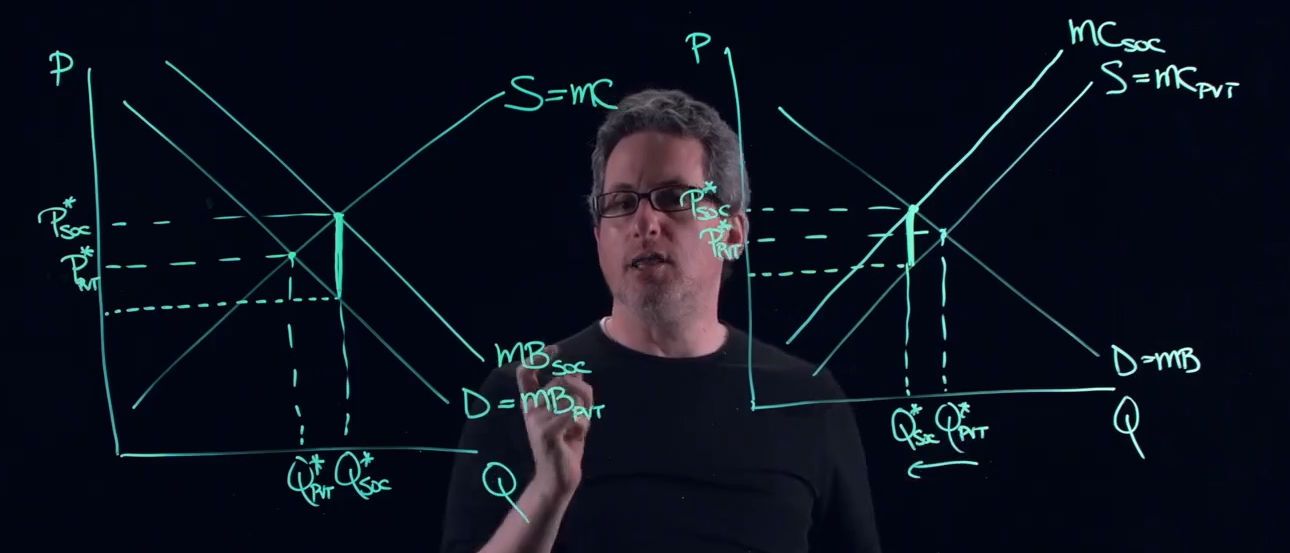
\includegraphics[width=0.5\textwidth]{Chapter16/externalities.png}
    \caption{Externalities}
    \label{fig:externalities}
\end{figure}
Every good or service can be described as rival in consumption or non-rival in consumption.\\
They are also excludable or non-excludable.\\
Excludable good means that you can prevent someone from using it.\\
Rival in consumption means that if you use it, I can't use it.\\
Most of what we look at it is excludable and rival in consumption.
\begin{figure}[H]
    \centering
    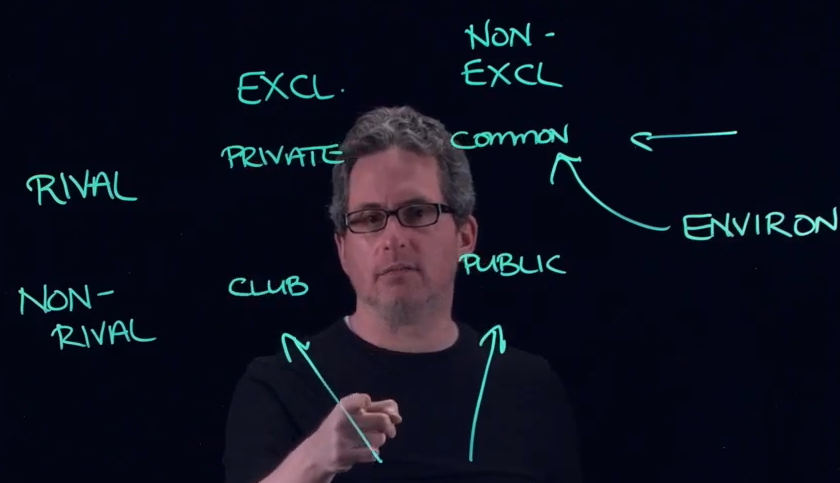
\includegraphics[width=0.5\textwidth]{Chapter16/Goods.png}
    \caption{Goods}
    \label{fig:goods}
\end{figure}
Club and public goods may require government intervention.\\
The government may provide subsidies for club goods.
\par
Public goods are characterized by free riding.\\
The government sums the individual demand curves vertically to get the market demand curve.\\
The issue is that the government does not know the individual demand curve sso they tax everyone.
\begin{figure}[H]
    \centering
    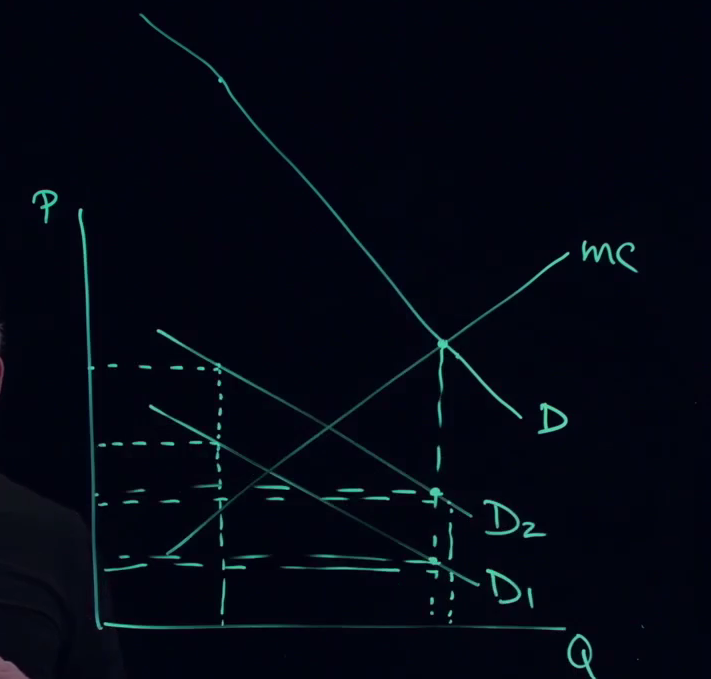
\includegraphics[width=0.5\textwidth]{Chapter16/PublicGoods.png}
    \caption{Public Goods}
    \label{fig:publicgoods}
\end{figure}
Information is excludable and non-rivalrous.\\
Knowledge is non-excludable and non-rivalrous.
\par
Asymmetric information is when one party knows more than the other party.\\
Two things come from this:
\begin{itemize}
    \item Adverse selection: occurs before a transaction takes place. 
    \item Moral hazard: occurs after a transaction takes place.
\end{itemize}
We deal with this by trying to symmetrize the information.